
\chapter{Resonance Search and Results} \label{chap:resonance}

The following chapter will discuss the details and results of a resonance 
search for an $A'$ in the mass range between 20 MeV/$c^2$ to 60 MeV/$c^2$.
This includes a discussion of the procedure used to determine if a significant
resonance was observed at a given $A'$ mass hypothesis and the statistical
formalism used to set an upper limit on both the signal and $A'$ coupling
strength.

This analysis makes use of
the unblinded portion of the 2015 HPS engineering run data which amounts to 
a luminosity of 74 nb$^{-1}$ (.4671 mC of charge) or 1/10 of a PAC day.  
A blind search for a resonance using the procedure outlined in this chapter 
and making use of the full 2015 engineering run 
dataset (1165.71 nb$^{-1}$, 7.2875 mC) is expected to be completed in the 
Summer of 2016.

\section{Searching for a Resonance}

If a heavy photon does indeed exist and has a mass that is within the acceptance
of the HPS detector, it will appear as a resonance above the copious QED trident
invariant mass distribution.  Such a signal is expected to be Gaussian in 
nature, with a mean equal to the mass of the $A'$, $m_{A'}$, and with a mass
dependent width, $\sigma_{m_{A'}}$, given by the mass resolution 
parameterization define in Section \ref{sec:mass_res}. With this in mind, the 
invariant mass distribution measured by HPS (see Chapter 
\ref{ch:event_selection} and Fig. \ref{fig:mass_selection}) will serve as the
starting point for this analyses. 
%In total, the invariant
%distribution contains 437,766 events binned into a histogram ranging between 
%0 and .1 GeV and bin sizes of 0.00005 GeV.
%\begin{figure}[t]
%    \centering
%    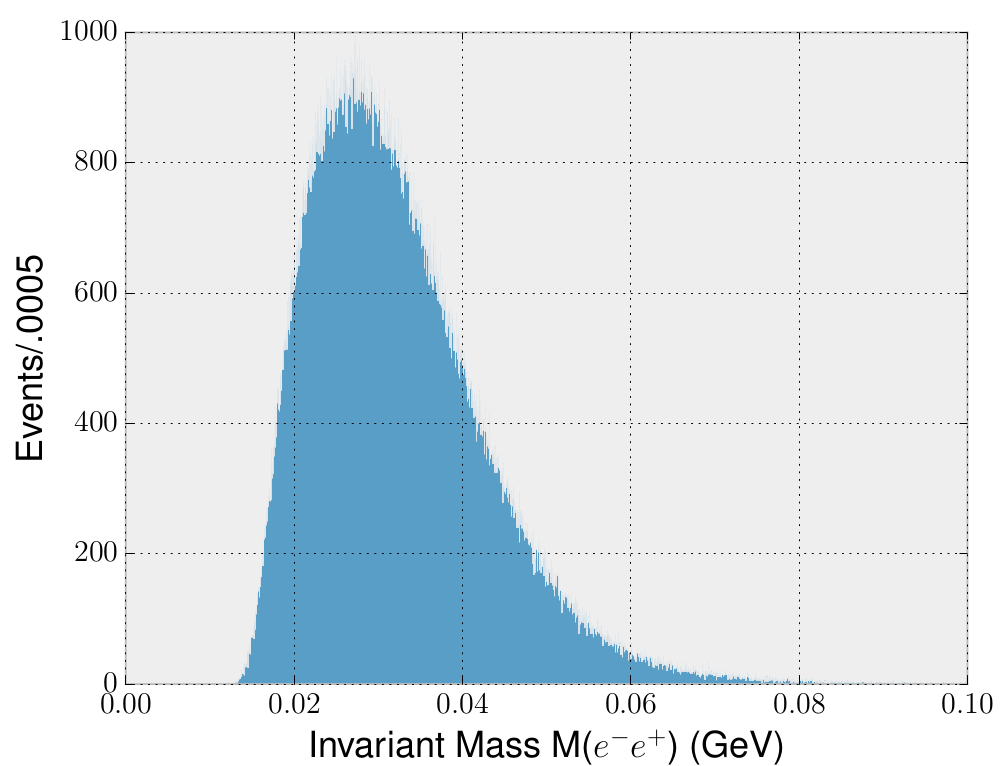
\includegraphics[width=1.0\textwidth]{images/invariant_mass_final.png}
%    \caption{The Heavy Photon Search $e^+e^-$ invariant mass distribution after
%             the final event selection has been applied.  The mass distribution
%             will serve as the starting point for the resonance search.}
%    \label{fig:mass_distribution}
%\end{figure}

\subsection{Maximum Likelihood Fit}

Since the mass of the $A'$ is unknown a priori, the 
$e^+e^-$ invariant mass spectrum needs to be scanned for any significant peaks.
Customarily, a search for a resonance is performed within a
window constructed around the mass hypothesis of interest.  Within the window,
the distribution of $A'$ signal events is modeled using the probability 
distribution function
\begin{equation}
    \begin{split}
    P(m_{e^+e^-}) 
        = 
        \mu \cdot \phi(m_{e^+e^-} | m_{A'}, \sigma_{m_{A'}}) + B\cdot p(m_{e^+e^-} | t_j)
    \end{split}
\end{equation}
where $m_{e^+e^-}$ is the $e^+e^-$ invariant mass, $\mu$ is the signal yield,
$B$ is the number of background events within the window, 
$\phi(m_{e^+e^-} | m_{A'})$ is a Gaussian probability distribution describing
the signal and $p(m_{e^+e^-} | t_j)$ is a Chebyshev polynomial of the first kind
with coefficients $t_j$ that is used to describe the background shape.
Estimating the 
signal yield as well the background normalization and shape within a window, can be
done by the method of maximum likelihood.  The theoretical formalism
used to do this will be outlined here but a detailed discussion can be found in
\cite{Cowan:2010js}.

Assume the events within the window are binned as $\mathbf{n} = (n_{1}, ... n_{i})$.
Furthermore, assume the center of the $i$th bin is given by $b_i$ and has a width
equal to $\epsilon$. 
The expected number of events of the $i$th bin is given by 
\begin{equation}
    E[n_i] = S_{i} + B_{i}
\end{equation}
where 
\begin{equation}
    S_{i} = \mu \int_{b_i - \epsilon/2}^{b_i + \epsilon/2} \phi(m_{e^+e^-} | m_{A'}, \sigma_{m_{A'}}) d (m_{e^+e^-})
\end{equation} 
\begin{equation}
    B_{i} = B_{total} \int_{b_i - \epsilon/2}^{b_i + \epsilon/2} p(m_{e^+e^-} | t_{j}) d (m_{e^+e^-}).
\end{equation}
Denoting the parameters that are not of immediate interest, i.e. the nuissance
parameters, by $\theta = (B_{total},  t_{j})$, an estimation
of $\mu$ and $\theta$ can be obtained by finding the parameters $\hat{\mu}$ and
$\hat{\theta}$ that maximize the Poisson likelihood function, $\mathcal{L}$
\begin{equation}
\mathcal{L}(\mu, \theta) = \prod_{k=1}^{n_{\text{bins}}} \frac{(S_{k} + B_{k})^{n_k}}{n_{k}!} e^{-(S_{k} + B_{k})}
\end{equation}
where the sum is over all bins within the window, $n_{\text{bins}}$.
In the case where the invariant mass is scanned for a resonance, the Poisson 
likelihood function is maximized within the window constructed around each
$A'$ mass hypothesis. This yields estimators for the signal yield and nuissance
parameters at each $A'$ mass hypothesis which are used to determine if a significant 
resonance was found.

\subsection{Likelihood Ratio} \label{sub:likelihood_ratio}

When searching for a resonance above a background distribution, it is 
necessary to discriminate between two scenarios:
\begin{itemize}
    \item The background only or null hypothesis, $H_{0}: \mu = 0$.
    \item The signal+background hypothesis or alternative, $H_{1}: \mu > 0$.
\end{itemize}
Establishing whether the signal+background model is significantly different 
from the background only model is typically done using the profile likelihood
ratio
\begin{equation}
    \lambda(\mu) = \frac{\mathcal{L}(\mu, \hat{\hat{\theta}})}{\mathcal{L}(\hat{\mu}, \hat{\theta})}
    \label{eqn:likelihood_ratio}
\end{equation}
where $\hat{\hat{\theta}}$ is the conditional estimator for the nuissance parameters 
obtained by maximizing the Poisson likelihood assuming that the null or 
background only hypothesis is true i.e. $\mu = 0$. The unconditional estimators $\hat{\mu}$ 
and $\hat{\theta}$ are obtained by maximizing the Poisson likelihood without
any constraints on $\mu$.
As can be seen from \ref{eqn:likelihood_ratio}, 
if the estimator of the signal yield, $\hat{\mu}$, is compatible (incompatible)
with the hypothesized $\mu$, the likelihood ratio will tend to 1 (0).

A more convenient test statistic is the log likelihood ratio defined as
\begin{equation}
    q_0 = \begin{cases}
            -2 \ln \frac{\mathcal{L}(0, \hat{\hat{\theta}})}{\mathcal{L}(\hat{\mu}, \hat{\theta})} 
            & \hat{\mu} > 0 \\
             0  & \hat{\mu} < 0.
        \end{cases}
\end{equation}
In the large sample limit, the test statistic
$q_0$ can be shown to follow a $1/2\chi^2$ distribution defined in \cite{Cowan:2010js} as 
\begin{equation}
    f(q_{0}|0) = \frac{1}{2} \left(\delta(q_{0}) + \frac{1}{\sqrt{2\pi}}\frac{1}{\sqrt{q_{0}}}e^{-q_0/2} \right)
    \label{eqn:half_chi}
\end{equation}
where the first term on the right side of the equation is a delta function at 0
and the second term is a $\chi^2$ distribution with one degree of freedom. 
%Equation \ref{eqn:half_chi} is simple the mixture 
%is asymptotically $1/2\chi^2$ \footnote{The 1/2 comes from the fact that only
%signal yields greater than 0 are being considered. See \cite{Cowan:2010js} for a 
%more detailed explanation.} distributed with degrees of freedom equal to the
%difference in parameters between the two models being tested.  In our current case, 
%the number of degrees of freedom is one, since the signal yield is the only 
%parameter that does not appear in
%the background only model.

Quantifying how extreme the observation is can be done by calculating a $p$-value as
\begin{equation}
    p = \int_{q_{0,obs}}^{\infty} f(q_{0} | 0) dq_{0}.
\end{equation} 
This is shown graphically on Fig. \ref{fig:p_value}.  Typically, the observed 
p-value is
\begin{figure}[t]
    \centering
    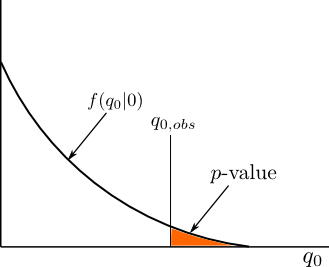
\includegraphics[width=.5\textwidth]{images/p_value.png}
    \caption{Graphical representation of a p-value.}
    \label{fig:p_value}
\end{figure}
compared against a significance level $\alpha$.  The significance level denotes
the probability of incorrectly rejecting the null hypothesis in favor of the 
alternative (type-I error).  In other words, it denotes the probability of there
being a statistical fluctuation in the background large enough to mimic a signal.  
If a $p$-value is 
found to be less than $\alpha$, the measurement is claimed to be significant. 
Typically, in particle 
physics, an $\alpha$ on the order of $3 \times 10^{-7}$ (5$\sigma$) is required
to claim discovery of new phenomena.  This means that there is a 1 in 
about 3.5 million chance that the observation is due to a fluctuation in the background.

\subsection{The Look-Elsewhere Effect}

As discussed previously in Section \ref{sub:likelihood_ratio}, a result is 
determined significant if the $p$-value is smaller than some pre-determined
threshold, $\alpha$.  However, 
when performing multiple test, as is the case when scanning a mass distribution
for a resonance, an observation with a $p$-value that is as extreme as $\alpha$
is bound to occur at a rate of $n\times\alpha$ where $n$ is the number of measurements.
This phenomena is known as the ``Look-Elsewhere Effect'' (LEE)
and needs to be taken into account through a correction to the ``local'' $p$-value
observed at each mass hypothesis.

Assuming that only a single heavy photon can be observed within the HPS invariant
mass distribution, the correction can be estimated using a large number
of pseudo-data sets and generating the distribution 
$f(q_{0, max} | 0)$ composed of the largest $q_{0}$ (i.e. smallest $p$-value)
from each of the invariant mass scans.
%The distribution $f(q_{0, max} | 0)$ can
%be derived by running a large number of pseudo-experiments and then calculating
%the $p$-value as was explained previously.
However, generating a distribution of $f(q_{0, max} | 0)$ that would allow 
an estimation of a ``global''  
$p$-value (i.e. local $p$-value after correction) down to the level of 5$\sigma$ with any accuracy would 
require running $> 10^{6}$ pseudo experiments.  Generating so many pseudo-data 
sets is often not feasible within a reasonable amount of time. 

Instead, the smallest
$p$-values obtained from a series of resonance searches on 10,000 pseudo
data sets were
ranked and the corresponding quantile was calculated \cite{Gross:2010qma}.  
A mapping from a local 
$p$-value to a global $p$-value is then created.  The mapping created 
for this analysis is shown on Figure \ref{fig:global_p_value}.
\begin{figure}[t]
    \centering
    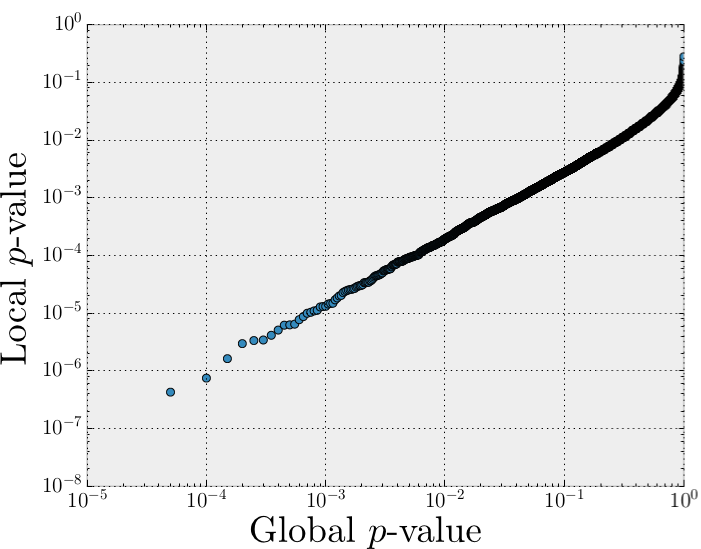
\includegraphics[width=\textwidth]{images/global_p_value_map.png}
    \caption{Mapping between local and global p-values.}
    \label{fig:global_p_value}
\end{figure}
As can be seen from the figure, a 
local $p$-value equal to 0.05 corresponds to a global $p$-value of $\sim$ 0.5.

\section{Fit Parameters}

Prior to performing the resonance search on real data, several fit parameters 
were optimized using pseudo data sets based on Monte Carlo.  These included the size of the fit 
window, the binning of the invariant mass distribution and the order of 
the polynomial used to describe the background.  All parameters were chosen 
such that signal yield pull
\begin{equation}
    \text{pull} = \frac{\mu_{\text{fit}} - \mu_{\text{inserted}}}{\mu_{\text{fit error}}}
\end{equation}
was minimized for all fits performed across an invariant mass spectrum.

\subsection{Pseudo Data Sets}

\begin{figure}[ht]
    \centering
    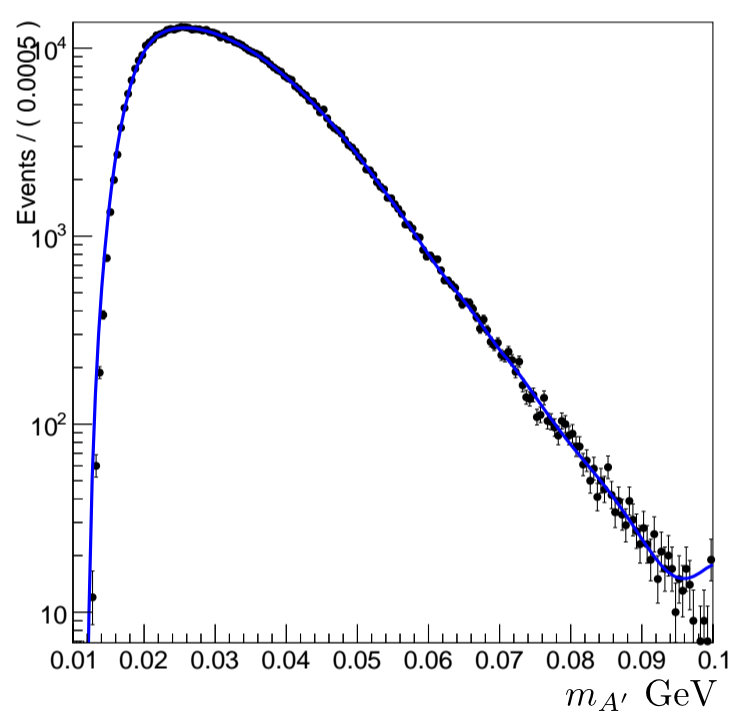
\includegraphics[width=0.7\textwidth]{images/smooth_pdf.png}
    \caption{Probability density function obtained by applying a smoothing algorithm 
             to the Heavy Photon Search Monte Carlo invariant mass distribution.}
    \label{fig:smooth_pdf}
\end{figure}

Pseudo data sets are needed to understand fitting systematics and to optimize
the fit function, window size and mass binning.  In order to obtain an invariant
mass probability
density function (PDF) that describes the data, smoothing algorithm 353 QH 
\cite{Friedman:1974vj} was
%What smoothing algorithm was used? Why? Was a K-S test used to make sure the
% resulting PDF matched the data set?
applied to the unit normalized final invariant mass MC distribution.  The resulting
PDF after smoothing (blue line) overlaid on top of the MC distribution it was generated 
from is shown on Fig. \ref{fig:smooth_pdf}.  

Pseudo data sets were then generated
by sampling the PDF between 0 and 100 MeV with the total number of
%events, 437,766,
events, 437,766, chosen to match the number observed in data.  The resulting
pseudo data is binned to match the data distributions with the expectation
value of each bin Poisson distributed.

%% What kind of sampling algorithm was used? 

\subsection{Mass Binning}

Ideally, an unbinned maximum likelihood fit would be used to estimate the fit 
parameters describe previously.  However, due to the large number of statistics, 
this wouldn't be possible to do in a reasonable amount of time.  Instead, 
a binned likelihood fit is performed with the bin size set such that the 
pulls are minimized.

In order to understand the effect of the bin size on the fitting systematics, 
pseudo data sets were binned using bin sizes of 0.2 MeV, 0.1 MeV and 0.05 MeV.
A resonance search was performed on each of the pseudo data sets and pull 
distributions were generated at 
%mean pull at
each mass hypothesis.
%was calculate.
Using this procedure, it was found that using
a bin size of 0.05 MeV minimizes the pulls, hence, it was used in the final
analysis.

\subsection{Fit Window and Polynomial Order}

The pseudo data sets were also used to understand what size fit window and what 
order polynomial minimizes the signal yield pulls. Performing a resonance search on 
each of the pseudo data sets using windows of size $n \times \sigma_{m_{A'}(m_{e^+e^-})}$
where $n$ is a scale factor, it was found that $n = 15$ minimizes the pulls 
across the whole range. Furthermore, it was found that the maximum window
size that could be used is 20 MeV after which the pulls would become worse. 
A similar procedure was used to determine the polynomial used to model the background.
It was found that a 7th order polynomial minimizes the pulls. 

\section{Results}

The resulting local $p$-values from a resonance search conducted in the range 
between 20 MeV and 60 MeV are shown on Fig. \ref{fig:local_p_values}. 
The most significant signal
was found at a mass of 27.525 MeV and has a local p-value of $4 \times 10^{-3}$.
The resulting signal plus background fit (blue) along with the signal component 
(red) and background component (green) is shown on Figure \ref{fig:fit_27}.
After correcting for the LEE, the corresponding global p-value is 
$\sim 10\%$.
\begin{figure}[t]
    \centering
    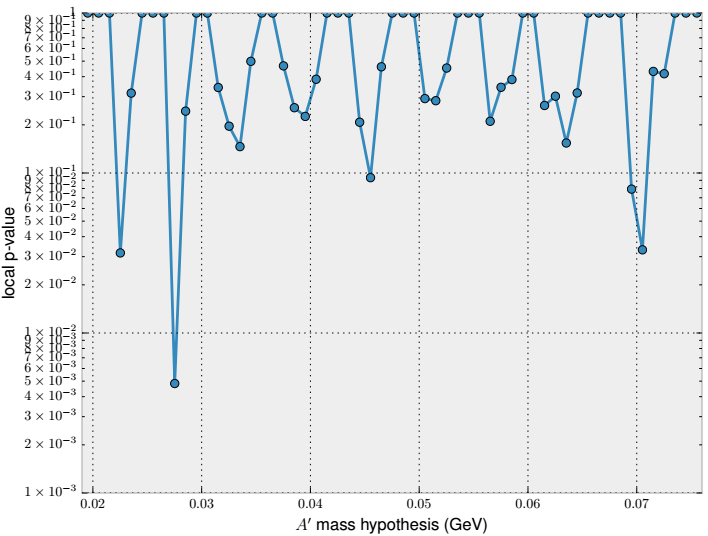
\includegraphics[width=\textwidth]{images/final_p_values.png}
    \caption{Resulting $p$-values from a resonance search for an $A'$ across the
    invariant mass spectrum.}
    \label{fig:local_p_values}
\end{figure}

\begin{figure}[ht]
    \centering
    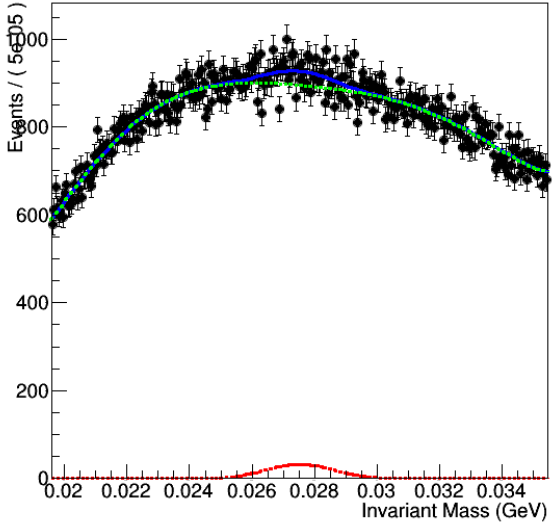
\includegraphics[width=.6\textwidth]{images/fit27.png}
    \caption{Resulting signal plus background fit (blue) assuming an $A'$ mass hypothesis
             of 27.525 MeV.  The signal component is shown in red while the 
         background component is shown in green.}
        
    \label{fig:local_p_values}
\end{figure}

\section{Setting Upper Limits on the Signal Yield}

Since no significant resonances were found, a 90\% confidence upper limit on the number
of signal events at each mass hypothesis was set.  For the purpose of setting
an upper limit, the likelihood ratio is inverted.  The statistic used
to set an upper limit is then
\begin{equation}
    q_{\mu} = \begin{cases}
        -2 \ln \frac{\mathcal{L}(\mu, \hat{\hat{\theta}})}{\mathcal{L}(0, \hat{\hat{\theta}})} 
            & \hat{\mu} < 0 \\
        -2 \ln \frac{\mathcal{L}(\mu, \hat{\hat{\theta}})}{\mathcal{L}(\hat{\mu}, \hat{\theta})} 
            & 0 \leq \hat{\mu} \leq \mu \\
             0  & \hat{\mu} > \mu
        \end{cases}
\end{equation}
with the corresponding $p$-value being given by
\begin{equation}
    p = \int_{q_{\mu,obs}}^{\infty} f(q_{\mu} | \mu) dq_{\mu}
\end{equation}
where $f(q_{\mu}|\mu)$ is the probability distribution of $q_{\mu}$ given the
hypothesized value of $\mu$. 
In order to find the upper limit, $\mu_{\text{up}}$, the test above is carried out over a range of
signal yields until a $p$-value of 0.1 (90\% confidence) is found.  The signal
yield value that corresponds to a $p$-value of 0.1 is $\mu_{\text{up}}$
and is often referred to as the unconstrained limit. 
%The value of
%$\mu_{\text{up}}$ found in this way
%is often referred to as the unconstrained limit.
The resulting 
unconstrained upper limits are shown in blue on Fig. \ref{fig:upper_limit}. 
\begin{figure}[t]
    \centering
    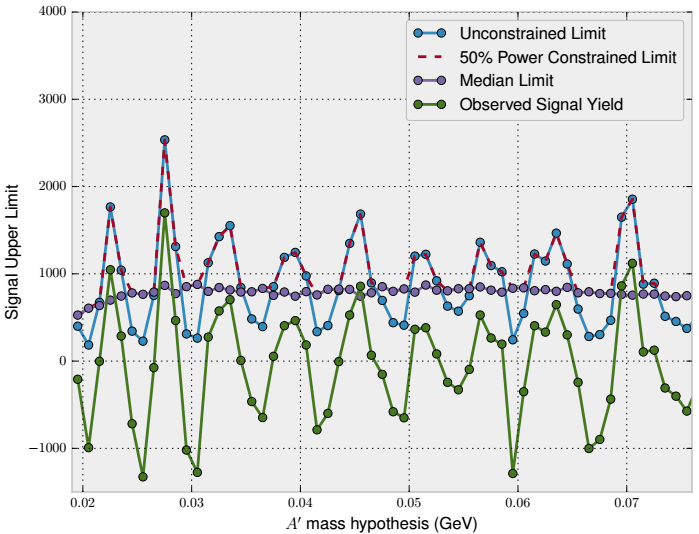
\includegraphics[width=\textwidth]{images/upper_limits.png}
    \caption{Upper limits on the signal yield at each mass hypothesis.}
    \label{fig:upper_limit}
\end{figure}

As shown in green on Fig. \ref{fig:upper_limit}, it is often the case that the
estimator for the signal yield, at a given mass hypothesis is zero or
even negative.  In such cases, the probability distribution function of the
test statistic $q_{\mu}$ assuming $\mu_{\text{up}}$ will nearly coincide with 
the distribution of $q_{\mu}$ assuming $\mu = 0$, i.e. the background only 
hypothesis.  As a result, there is a lack of 
sensitivity to a signal measurement at those mass hypothesis.

In such cases, a 50\% power-constrained upper limit on the signal is set
\cite{Cowan:2011an}.
At each mass hypothesis, a distribution of signal upper limits is generated from
background only pseudo-data sets and the median (50\% quantile) upper limit
is calculated, $\mu_{\mbox{median}}$. The upper limit in that region is then set to 
the larger of either the unconstrained limit or the median limit
\begin{equation}
    \mu_{pc} = \mbox{max}(\mu_{\text{up}}, \mu_{\text{median}}).
\end{equation}
The power constrained limits are shown in red on Fig. \ref{fig:upper_limit}.

\section{Setting a limit on $\epsilon$}

As discussed in chapter 2, the kinematic similarities between heavy photons and 
radiatives allows their cross sections to be related within a mass window, 
$\delta m$, near $m_{A'}$ as 
\begin{equation}
    \frac{d\sigma(e^-Z \rightarrow e^-A'Z(A' \rightarrow e^+e^-))}{
    d\sigma(e^-Z \rightarrow e^-\gamma^*Z(\gamma^* \rightarrow e^+e^-))} = 
    \left( \frac{3 \pi \epsilon^2}{2 N_{eff} \alpha} \right)
        \left( \frac{m_{A'}}{\delta m_{A'}} \right)
    \label{eqn:ap_rad_xsec}
\end{equation}
where $N_{eff}$ is the number of available decay channels available.  For the 
$A'$ masses considered in this analysis, $N_{eff} = 1$. Using equation 
\ref{eqn:ap_rad_xsec}, the upper limit on the signal, $S_{\text{up}}$, can be related to an
upper limit on the $A'$ coupling strength as 
\begin{equation}
    \epsilon^2 = \left (\frac{S_{\text{up}}/m_{A'}}{
                f\Delta B/\Delta m} \right) 
                \left(\frac{2 N_{eff} \alpha}{3 \pi} \right)
    \label{eqn:eps}
\end{equation}
where $\Delta B/\Delta m$ is the number of 
background events per MeV and $f$ is the ratio of the pure radiative cross-section to the full trident 
cross section.  The ratio is calculated using MC and is shown on Figure \ref{fig:rad_frac} as 
a function of mass.
In order to calculate the number of background 
events per MeV, a 1 MeV window is constructed around the $A'$ mass hypothesis
and the number of background events in that window are counted.  The resulting 
number of background events per MeV at each mass hypothesis are shown on Fig. 
\ref{fig:background_mev}.  

The limits on the coupling strength derived using equation \ref{eqn:eps}
are shown on Fig. \ref{fig:epsilon_upper_limit}. Using the full data set
the reach is expected to increase by a factor of ~4 down to $\epsilon^2 \sim 10^{-6}$.
\begin{figure}[ht]
    \centering
    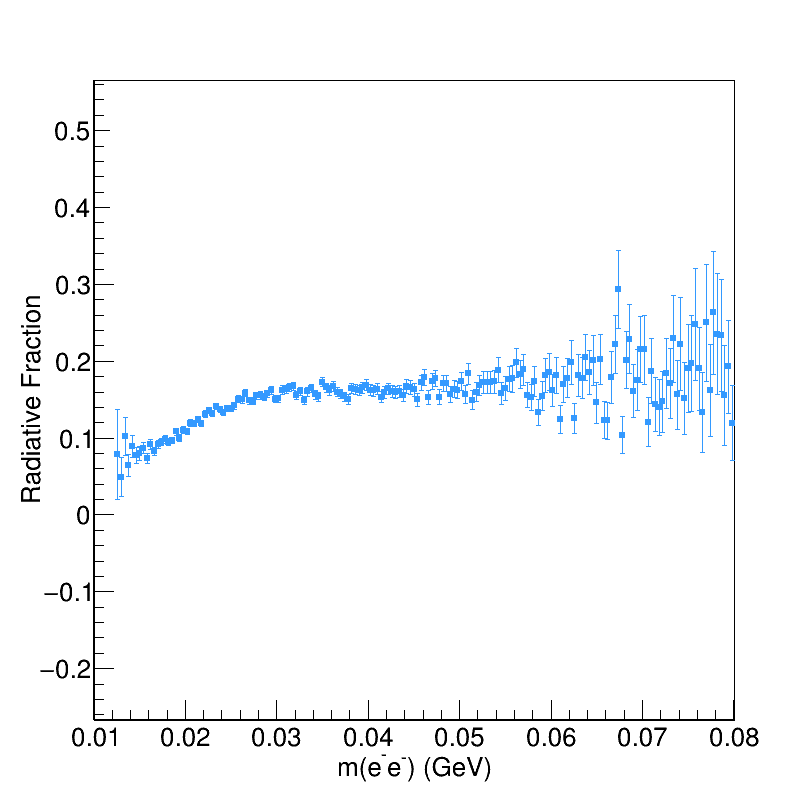
\includegraphics[width=.8\textwidth]{images/rad_frac.png}
    \caption{The ratio of the pure radiative cross-section to the full trident 
             cross section as a function of mass.}
    \label{fig:rad_frac}
\end{figure}
\begin{figure}[hb]
    \centering
    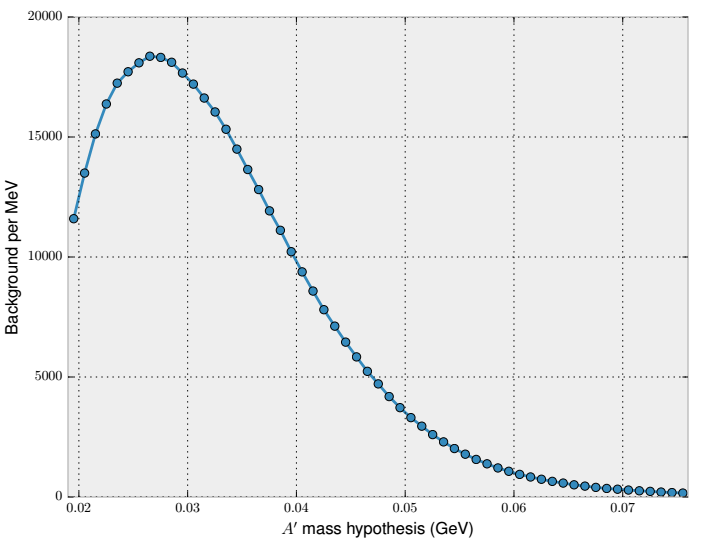
\includegraphics[width=\textwidth]{images/bkg_mev.png}
    \caption{The number of background events in a 1 MeV window around each $A'$ mass hypothesis.}
    \label{fig:background_mev}
\end{figure}
\begin{figure}[ht]
    \centering
    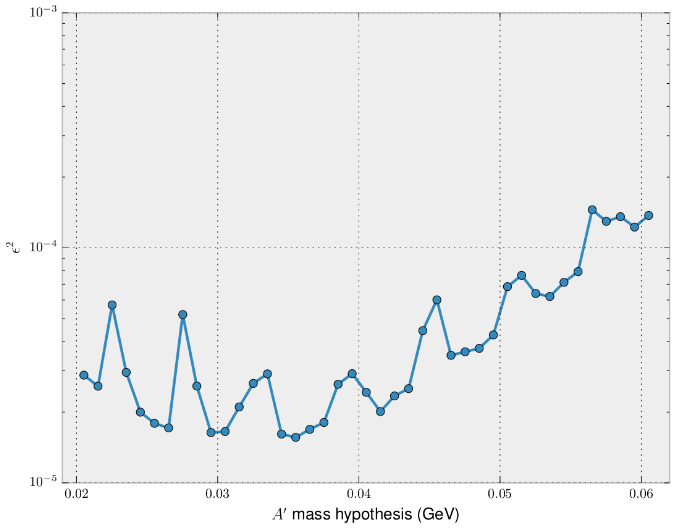
\includegraphics[width=\textwidth]{images/final_coupling_upper_limits.png}
    \caption{Upper limits on the coupling strength.}
    \label{fig:epsilon_upper_limit}
\end{figure}





